\section{The Socratic method}
\label{sec:socratic}

The Socratic method is a questioning technique used in teaching and philosophy to encourage critical thinking and self-discovery \cite{SocraticMethidWiki}. The method involves asking a series of questions to explore complex ideas and help individuals arrive at their own understanding of a concept. It is based on the belief that knowledge cannot be simply imparted, but must be discovered through a process of questioning and dialogue.


Some of the Socratic method's key principles and guidelines to conduct critical thinking include:
\begin{noindlist}
\item Posing open-ended questions: The teacher or facilitator starts with a question to stimulate thinking and draw out ideas.
\item Clarifying key terms: The teacher helps the students clarify and define relevant terms and concepts to ensure everyone is on the same page.
\item Providing examples and evidence: The teacher or facilitator encourages the students to provide examples and evidence as reasons to support their claims.
\item Challenging reason-to-conclusion argument: The teacher or facilitator challenges the students' arguments and encourages them to question their own beliefs and to consider alternative perspectives.
\item Summarizing and drawing conclusions: The teacher helps the students summarize and draw conclusions from the discussion.
\item Reflecting on the process: The teacher and students reflect on the effectiveness of the method and what they learned through the dialogue.
\end{noindlist}

These principles of the Socratic method are realized through various methods and strategies. (Note the term ``method'' are used at the abstract level referring to the Socratic teaching
through questioning method, and his specific questioning techniques.) Some well-known examples of the Socratic method in action include Plato's ``Dialogues'' and ``Republic'' \cite{PaltoRepublicURL}, where Socrates uses questioning to  explore complex ideas and stimulate critical thinking in his interlocutors.

%\noindent
%\setlength{\leftskip}{-\parindent}
\begin{noindenumerate}
\item Definition: Socrates is known for his use of definition to clarify and explain the meaning of key terms and concepts.
\item Generalization: This method draws general principles from patterns that underlie observations and theories.
Generalization is used to form more certain and comprehensive conclusions.

\item Induction: Similar to generalization, but induction is based only on empirical evidence. Inductive reasoning provides hypotheses with high uncertainty.

\item Elenchus: This method involves cross-examination, where a series of questions is used to test the consistency and coherence of hypotheses and beliefs. Elenchus aims to 
test the validity of someone's arguments and to help them refine their thinking and eventually come up with well-supported hypotheses.

\item Hypothesis Elimination: This method involves eliminating false hypotheses and beliefs by testing them against counterexamples and logical reasoning.  Different from method elenchus, hypothesis elimination tests a hypothesis against evidence and logic to determine if it is true or false. 

\item Maieutics: This method involves helping individuals bring out the knowledge and understanding they already possess.
Maieutics is conducted by asking questions that encourage the person to reflect on their own experience, knowledge, beliefs and to explore alternative perspectives. Maieutics fosters  self-discovery, creative writing, and innovation.

\item Dialectic: This method involves exploring opposing viewpoints through dialogue or debate to arrive at a deeper understanding of a subject.

\item Recollection: This method involves the belief that knowledge is innate, and that people can remember what they already know through a process of questioning.

\item Irony: This method involves exposing ignorance and pretensions through irony, and pointing out the gap between claims and true understanding.

\item Analogy: This method involves comparing and contrasting different concepts through analogies, in order to help individuals understand complex ideas.
\end{noindenumerate}

%\subsection{Choices of Methods for Prompt Engineering}

At first glance, some reasoning methods may seem similar. For example, both induction and generalization use inductive reasoning, while both elenchus and hypothesis elimination use deductive reasoning. Similarly, methods like definition and dialectic use both inductive and deductive reasoning to explore opposing viewpoints through dialogue or debate. However, it is important to note that these methods have distinct differences, which will be discussed later in this paper.

In the context of critical thinking, methods like definition, elenchus, dialectic, hypothesis elimination, and generalization play active roles. On the other hand, during the brainstorming stage or in the context of creative thinking, methods like maieutics, induction, and counterfactual thinking are more relevant.

Analogy, irony, and recollection, are less relevant to our goal, so we do not consider them. Irony and analogy may not be necessary when working with language models, as these models may not understand figurative language. Recollection is limited by the memory of ChatGPT and GPT-3, which is a context window of $4k$ and $8k$, respectively. The prompter must use this limited space as context to allow the language model to recall information.


\begin{comment}
To improve input specificity, we suggest using the dialectic method with definition. The method of maieutics, combined with generalization and induction strategies, can be used to adapt a prompt template to the strengths of an LLM. The hypothesis elimination method can be used by all methods to remove information from low-reliability sources. Furthermore, we propose the addition of counterfactual reasoning \cite{NormTheory1986,FuncTheoryCounterfactual2008} to the list of methods. Counterfactual reasoning involves considering alternate outcomes of events, and the Socratic method can be used to guide discussions on this topic by encouraging critical thinking and self-reflection.
\end{comment}

\subsection{Illustrative Critical Reading Example}

To illustrate how these methods can practically be applied, let's use the example of critical reading. Critical reading is a crucial component of critical thinking, which involves evaluating the quality and credibility of written materials, from research papers to blog posts \cite{lai-etal-2017-race,PaulBinkerCT1990}. It requires a systematic and analytical approach, asking relevant questions, and using effective prompts to gain deeper understanding of the text \cite{Elder2010}.


\begin{table}[ht!]
%\vspace{-.1in}
\begin{center}
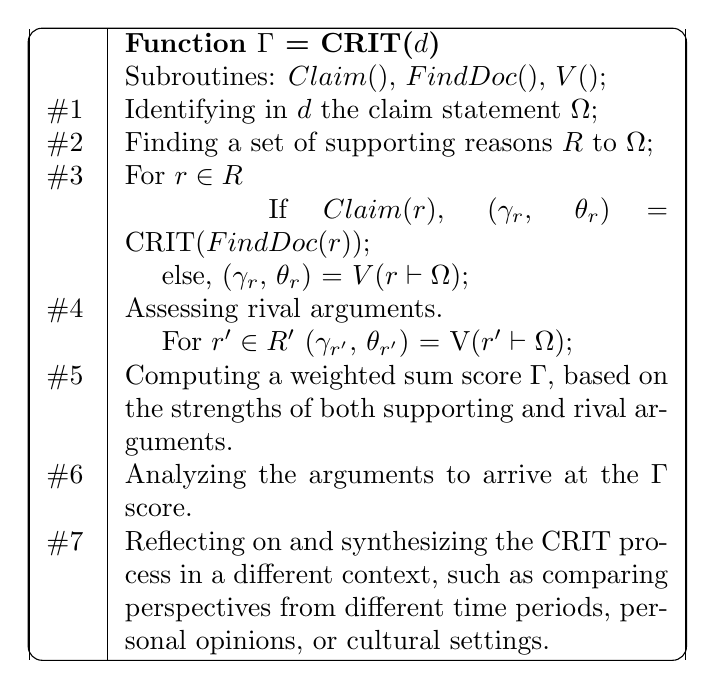
\begin{tikzpicture}
\node (table) [inner sep=0pt] {
\begin{tabular}{|p{0.56cm}|p{6.9cm}|}
\toprule
\textbf{} & \textbf{Function $\Gamma$ = CRIT($d$)} \\
\midrule
%& Function $\Gamma$ = CRIT($d$); \\
& Subroutines: $Claim$(), $FindDoc$(), $V$(); \\
\#1 & Identifying in $d$ the claim statement $\Omega$; \\
\#2 & Finding a set of supporting reasons $R$ to $\Omega$; \\
\#3 & For $r \in R$ \\
& ~~~~{If} $Claim$($r$), ($\gamma_r$, $\theta_r$) = CRIT($FindDoc$($r$)); \\
& ~~~~{else}, ($\gamma_r$, $\theta_r$) = $V$($r \vdash \Omega$); \\
\#4 & Assessing rival arguments. \\
& ~~~~For $r' \in R'$ ($\gamma_{r'}$, $\theta_{r'}$) = V($r' \vdash \Omega$); \\
\#5 & Computing a weighted sum score $\Gamma$, based on the strengths of both supporting and rival arguments. \\
\#6 & Analyzing the arguments to arrive at the $\Gamma$ score. \\
\#7 & Reflecting on and synthesizing the CRIT process in a different context, such as comparing perspectives from different time periods, personal opinions, or cultural settings. \\
\bottomrule
\end{tabular}
};
\draw [rounded corners=.5em] (table.north west) rectangle (table.south east);
\end{tikzpicture}
\end{center}
\caption{CRIT Pseudo-code. Input $d$ document, output $\Gamma$ validation score, V() validation routine, $R$ reason set, $R'$ rival reason set, ($\gamma_{r}$, $\theta_{r}$) validity and credibility scores of $r \vdash \Omega$.}
\label{tab:CRIT}
%\vspace{-.2in}
\end{table}


To aid in critical reading, we introduce a template called CRIT, which stands for Critical Reading Inquisitive Template. Given a document $d$, CRIT evaluates it and produces a validation score $\Gamma$. Let $\Omega$ denote the conclusion or claim of $d$, and let $R$ be the set of reasons supporting the claim. We define ($\gamma_r, \theta_r$) = V($r \vdash \Omega$) as the causal validation function, where $\gamma_r$ denotes the validation score $\theta_r$ the source credibility score and for each reason-to-conclusion entailment $r \vdash \Omega$. Table~\ref{tab:CRIT} presents the pseudo-code of $\Gamma$ = CRIT($d$), which generates the final validation score for document $d$ with justifications.

In the following sections, we will discuss five methods: 1) definition, 2) elenchus, 3) dialectic, 4) maieutics, and 5) counterfactual thinking.


\subsection{Method of Definition}

As shown in the pseudocode in Table~\ref{tab:CRIT}, 
the CRIT algorithm starts in
its step $\#1$, asking GPT-3 to identify the conclusion of a document. To avoid any misunderstandings, the prompt includes a clear instruction and definition. (In the square brackets, {\em in} denotes a input slot to an LLM and {\em out} the output slot.)

\begin{table}[ht!]
\small
\begin{tabular}{p{0.6cm}|p{7.2cm}}
p1.1 & ``What is the conclusion in document [in: $d$] 
  [out: $\Omega$]? \\ 
& The conclusion statement may 
  be written in the last paragraph, near 
  keywords "in conclusion," "in summary," or "therefore."'' \\
\end{tabular}
\end{table}

We can use
the {\em definition} method to 
improve the understanding of the document. 
One approach is paraphrasing the prompt 
into multiple prompts and grouping them into an ensemble, similar to forming a thesis committee. (Section~\ref{sec:template} presents
prompt ensemble in details.)
Different members can phrase the same question in different ways or ask it from a different perspective.  For example:

\begin{table}[h!]
\small
\begin{tabular}{p{0.6cm}|p{7.2cm}}
p1.2 &  ``What is the issue addressed by [in: $d$] 
  [out: $\Omega$]?'' \\
p1.3 & ``What is the most important outcome presented in text [in: $d$]? [out: $\Omega$]''
\end{tabular}
\end{table}

Step $\#2$ in Table~\ref{tab:CRIT} prompts 
GPT-3 to find a set of
supporting reasons.  Similarly, the prompt can
be ``evidences'', ``opinions'', in addition to
``reasons'' to query for the document's 
support to its conclusion.

\begin{table}[ht!]
\small
\begin{tabular}{p{0.6cm}|p{7.2cm}}
p2 & ``What are the supporting reasons [out: $R$] of conclusion \\
& [in: $\Omega$] of [in: $d$]?'' 
\end{tabular}
\end{table}

\begin{comment}
Note that prompts can be submitted all together or
one-by-one to GPT-3. Our empirical study 
on reading comprehension
samples~\cite{501Q2004} shows that issuing prompts one-by-one
generates output with finer details.  This is because
GPT-3 has a chance to examine a document multiple times
for slightly different purposes.
For teaching K-12 students critical reading, 
the one-by-one prompting is
better because it allows students to interact with
CRIT step-by-step.  
\end{comment}

\subsection{Method of Elenchus}

The method of elenchus is rooted in the Greek word ``elenchein,'' which translates to examine. This method involves cross-examining the results generated by GPT-3 to evaluate the consistency and coherence of the arguments. The goal is to arrive at a deeper understanding of the validity of the reasons and conclusion, and to identify any potential weaknesses or flaws in the arguments.

Step $\#3$ of the CRIT algorithm (in Table~\ref{tab:CRIT}) prompts GPT-3 to assess the validity of each reason $r \in R$ as justification for the conclusion $\Omega$ through the function V($r \vdash \Omega$). To validate the reason-to-conclusion argument, CRIT must evaluate the presented reason and its causal relationship with the conclusion and conduct cross examination, which is precisely the task of the method of elenchus.

CRIT issues four prompts to evaluate the logic validity and source credibility of the $r \vdash \Omega$ entailment. Prompt $\#3.2$ elicits supporting evidence for reason $r \in R$. This evidence can be a theory, an opinion, statistics, or a claim from other sources. If the reasoning is a claim, then the sources that the claim is based on are recursively examined. The strength of the argument and its source credibility are rated on a scale of $1$ to $10$, with $10$ being the strongest.


\begin{table}[h!]
\small
\begin{tabular}{p{0.6cm}|p{7.2cm}}
p3.1 & ``What is the evidence for reason [in: $r$] to support
conclusion [in: $\Omega$] in document [in: $d$]? [out: evidence]'' \\ 
p3.2 & ``What is the type of evidence? A) a theory, B) an opinion, C) statistics, or {\color{red}D}) a claim from other sources?'' \\
p3.3 & ``If the evidence of reason [in: $r$] is {\color{red}D}),
  call CRIT recursively to extract supporting reasons [out: $R'$].'' \\
p3.4 & ``How strongly does reason [in: $r$] support
  [in: $\Omega$] in document [in: $d$]? Rate argument validity [out: $\gamma_v$] and source credibility [out: $\gamma_c$] between $1$ and $10$ (strongest).''
\end{tabular}
\end{table}


It may be beneficial to also incorporate the counter-argument method in order to gain a more comprehensive and balanced evaluation of the argument. This can result in a deeper understanding of the topic being discussed. We will be discussing this further in the next section.

\begin{comment}
\begin{table}[h!]
\small
\begin{tabular}{p{0.6cm}|p{7.2cm}}
\end{tabular}
\end{table}
\end{comment}

\subsection{Method of Dialectic}

The easiest way to mislead without lying outright is to leave out critical counterarguments from the reader.
CRIT relies on GPT-3 to generate and
evaluate counter arguments, similar to
how it prompts GPT-3 to extract and 
evaluate reasons. 

CRIT in its step $\#4$ asks GPT-3 to provide missing
rival reasons, and then pair rival reasons
with the conclusion to conduct validation.
There are two strategies to 
bring counter arguments to the surface.
The first strategy attacks the weakest 
arguments with the lowest scores and asking
GPT-3 to attack those entailment's.

\begin{table}[h!]
\small
\begin{tabular}{p{0.6cm}|p{7.2cm}}
p4 & ``Are there counter counterargument against [in: $r \vdash \Omega$] in [in: $d$]? If so, provide counter reasons [output $R'$].''
\end{tabular}
\end{table}

For finding omitted information, CRIT can
query GPT-3 without quoting any $r \in R$,
and follow the same process. At the end,
CRIT can append to the $\gamma$ score with
a $-\gamma$ score, and provide 
an alert to the reader with a 
a summary of the counter argument. 

Finally, in step $\#5$, CRIT computes an aggregated 
score by performing a weighted sum on
the validation multiplied by credibility score,
of both arguments and counter arguments, and then
output the final assessment score $\Gamma$.

\begin{table}[h!]
\small
\begin{tabular}{p{0.6cm}|p{7.2cm}}
p5 & ``Final score [out: $\Gamma$]. $\Gamma = 
\sum_{r \in R \cup R'} \gamma_r \times \theta_r / |R \cup R'|$.
\end{tabular}
\end{table}
%\noindent
%\subsubsection*{Remarks on Critical Reading vs. Thinking} 
%\hfill \break



\subsection{Method of Maieutics}
\label{sec:Maieutics}

The maieutic method derives from the Greek word ``maieutikos,'' meaning midwife. It is founded on the belief that a teacher's role is to facilitate students in bringing forth their own understanding of a subject, rather than simply conveying knowledge. Unlike the elenctic method, which aims to detect and eliminate false hypotheses, maieutics centers on helping students reveal their own understanding of a subject. In this dialogical method, the teacher asks questions that are intended to guide the student in discovering their own comprehension, rather than providing them with information or answers.

Moving on to GRIT, after the text has been scored in step $\#5$, it is valuable for readers or students to summarize and analyze the justifications produced by GPT-3 to enhance their analytical and writing skills. CRIT can prompt GPT-3 for a report, and then readers and students can compare their notes.

\begin{table}[h!]
\small
\begin{tabular}{p{0.6cm}|p{7.2cm}}
p6 & ``For every $r \in R \cup R'$ justify the validity score $\gamma_r$ and source credibility score $\theta_r$ for
each entailment $r \vdash \Omega$.''
\end{tabular}
\end{table}


\subsection{Counterfactual Reasoning}
\label{sec:cf}

Counterfactual reasoning~\cite{Cross-Examination2021,WinArgument2006} can be seen as a natural extension of the Socratic method, as both involve questioning assumptions and exploring alternative perspectives. 
Counterfactual thinking involves imagining alternative scenarios to what actually happened, often using phrases like ``what if'' or ``if only.''
By incorporating counterfactual reasoning into prompt engineering, one can facilitate exploration of alternative possibilities and promote more nuanced and complex understanding of a given topic.

The final step of GRIT involves using the counterfactual method to encourage students to reconsider the arguments and counterarguments presented in the text based on new contextual information. CRIT can prompt students with questions such as ``what if the debate in the text took place now instead of in the 1950s?'' or ``what if the main event in the text occurred in Asia instead of in Europe?'' Students can express their own opinions and findings based on further reading and statistics, and challenge the conclusions drawn in the text. Table~\ref{tab:CRIT} lists three contexts for consideration: when, who, and where.


\subsection{Remarks on the Socratic Method and CRIT}

As we have shown that for critical reading,
GRIT uses three methods, definition, elenchus, and dialectic.  
For critical thinking, CRIT uses methods maieutics and counterfactual reasoning. For more explorative 
thinking, 
methods such as induction can be used for informal brainstorming, hypothesis elimination for removing weak propositions, and generalization for deriving principles from examples.

Please note that prompts can be submitted to GPT-3 either all together or one-by-one. Our empirical study on reading comprehension samples~\cite{501Q2004} demonstrates that issuing prompts one-by-one results in outputs with finer details. This is because GPT-3 has the opportunity to analyze a document multiple times for slightly different purposes. For teaching critical reading to K-12 students, one-by-one prompting is preferred as it allows students to engage with CRIT step-by-step.

\begin{comment}
\begin{small}
\begin{verbatim}
\end{verbatim}
\end{small}
\end{comment}

